\documentclass[12pt]{article}
% \documentclass{article}
\usepackage{amsmath}
\usepackage{graphicx,subfigure}
\usepackage{caption}
\usepackage[scheme=plain]{ctex}
\pagestyle{empty}
\usepackage{amsmath,times,bm,hyperref}
\usepackage{amssymb}
\usepackage{listings}
\usepackage{xcolor}
\lstset { %
    language=C++,
    backgroundcolor=\color{black!5}, % set backgroundcolor
    basicstyle=\footnotesize,% basic font setting
}



%%%%%%%%%%%%%%%%%%%%%%%%%%%%%%%%%%%%%%%%%%%%%%%%%%
% Do not modify the dimensions of the page
\setlength{\topmargin}{0mm}
\setlength{\headheight}{0mm}
\setlength{\headsep}{0mm}
%% 25.4 -25.4 = 0
\setlength{\topmargin}{0mm}
%% 25.4 -25.4 = 0
\setlength{\oddsidemargin}{0mm}
%% 210 -25(left) -25(right) = 160
\setlength{\textwidth}{160mm}
%% 297 -25(top) -30(bottom) = 242
\setlength{\textheight}{242mm}
\setlength{\parindent}{0pt}
\setlength{\parskip}{12pt}
% Do not modify the dimensions of the page
%%%%%%%%%%%%%%%%%%%%%%%%%%%%%%%%%%%%%%%%%%%%%%%%%%

\begin{document}

\title{\bf MAE5032 Final Project}
\author{Qiang Li}
\date{\today}
\maketitle

\section*{1. Problem}
We consider the transient heat equation in a one-dimensional (1D) domain $\Omega := (0,1)$. The boundary of the domain is $\Gamma = \left\lbrace 0, 1 \right\rbrace$.
Let $f$ be the heat supply per unit volume, $u$ be the temperature,  $\rho$ be the density, $c$ be the heat capacity, $u_0$ be the initial temperature, $\kappa$ be the conductivity, $n_x$ be the Cartesian components of the unit outward normal vector . The boundary data involves the prescribed temperature $g$ on $\Gamma_g$ and heat flux $h$ on $\Gamma_h$. The boundary $\Gamma$ admits a non-overlapping decomposition: $\Gamma = \overline{\Gamma_{g} \cup \Gamma_h}$ and $\emptyset = \Gamma_g \cap \Gamma_h$. The transient heat equation may be stated as follows.

\begin{align*}
\rho c \frac{\partial u}{\partial t} - \kappa  \frac{\partial^2 u}{\partial x^2} &= f \quad \mbox{ on } \Omega \times (0,T) \\
u &= g \quad \mbox{ on } \Gamma_{g} \times (0,T) \\
\kappa \frac{\partial u}{\partial x} n_{x}  &= h \quad \mbox{ on } \Gamma_h \times (0,T) \\
u|_{t=0} &= u_0 \quad \mbox{ in } \Omega.
\end{align*}

\section*{2. Theoretical analysis}
\subsection*{2.1 Explicit Euler method}
\begin{equation}
    \frac{\partial u}{\partial t}=\frac{u^{n+1}-u^n}{\Delta t}+O(\Delta t^2)\label{partial time}
\end{equation}
\begin{equation}
    \frac{\partial^2 u}{\partial x^2}=\frac{u_{i+1}-2u_i+u_{i-1}}{\Delta x^2}+O(\Delta x^3)\label{partial u}
\end{equation}
With FDM, the transient heat equation in 1D can be dispersed into the following:
\begin{equation}
    u^{n+1}=u^n+\frac{\kappa\Delta t}{\rho c\Delta x^2}(u_{i+1}^n-2u_i^n+u_{i-1}^n)+\frac{f\Delta t}{\rho c}
\end{equation}

So we can get a tri-diagonal system $AX+X1=b$:
\begin{center}
\begin{pmatrix}
b & a & 0 & ... & 0 \\
a & b & a \\
 & & ... & \\
 &  & a & b & a\\
0 & 0 & ... & a & b
\end{pmatrix}\begin{pmatrix}
u_1^{n} \\
u_2^{1} \\
. \\
. \\
u_m^{n}
\end{pmatrix}+$\frac{f\Delta t}{\rho c}$=\begin{pmatrix}
u_1^{n+1} \\
u_2^{n+1} \\
. \\
. \\
u_m^{n+1}
\end{pmatrix}
\end{center}
\begin{equation*}
    a=\frac{\kappa\Delta t}{\rho c\Delta x^2}, b=1-2\frac{\kappa\Delta t}{\rho c\Delta x^2}
\end{equation*}


\subsection*{2.2 Implicit Euler method}
From eq. \ref{partial time} and eq. \ref{partial u}, we can deduce the following:
\begin{equation}
    \rho c\frac{u_i^{n+1}-u_i^n}{\Delta t}-\kappa\frac{u_{i+1}^{n+1}-2u_i^{n+1}+u_{i-1}^{n+1}}{\Delta x^2}=f
\end{equation}
\begin{equation}
    -\frac{\kappa\Delta t}{\rho c\Delta x^2}u_{i+1}^{n+1}+(1+2\frac{\kappa\Delta t}{\rho c\Delta x^2})u_i^{n+1}-\frac{\kappa\Delta t}{\rho c\Delta x^2}u_{i-1}^{n+1}=u_i^n+\frac{f\Delta t}{\rho c}
\end{equation}

So we can get a tri-diagonal system $AX=b$:
\begin{center}
\begin{pmatrix}
b & a & 0 & ... & 0 \\
a & b & a \\
 & & ... & \\
 &  & a & b & a\\
0 & 0 & ... & a & b
\end{pmatrix}\begin{pmatrix}
u_1^{n+1} \\
u_2^{n+1} \\
. \\
. \\
u_m^{n+1}
\end{pmatrix}=\begin{pmatrix}
u_1^n+\frac{f\Delta t}{\rho c} \\
u_2^n+\frac{f\Delta t}{\rho c} \\
. \\
. \\
u_m^{n}+\frac{f\Delta t}{\rho c}
\end{pmatrix}\\
 \end{center}
\begin{equation*}
    a=-\frac{\kappa\Delta t}{\rho c\Delta x^2}, b=1+2\frac{\kappa\Delta t}{\rho c\Delta x^2}
\end{equation*}

\subsection*{2.3 Exact solution}
Because $\frac{\partial u}{\partial t}=0$ , so we can get exact solution by integration.
\begin{equation}
    u_{exact} = \frac{sin\pi x}{\pi^2}
\end{equation}

\subsection*{2.4 Stability analysis}

\section*{3. Code analysis}
\begin{figure}
    \centering
    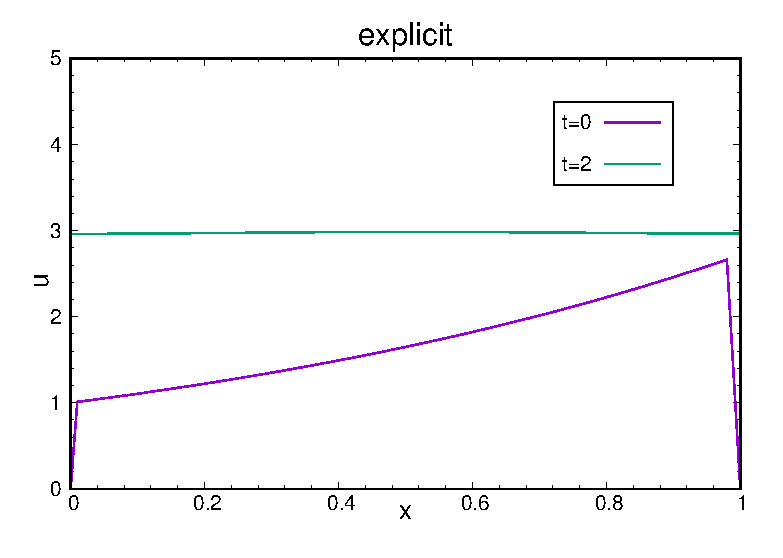
\includegraphics{../plot/explicit.eps}
    \caption{explicit scheme result}
    \label{fig:explicit}
\end{figure}

\begin{figure}
    \centering
    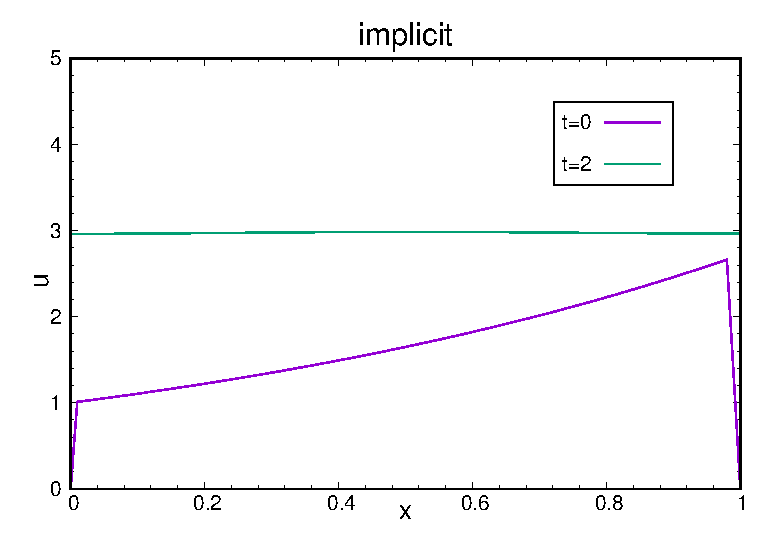
\includegraphics{../plot/implicit.eps}
    \caption{implicit scheme result}
    \label{fig:implicit}
\end{figure}

\subsection*{3.1 Code result}
Fig \ref{fig:explicit} and Fig \ref{fig:implicit} are the results after calculating 100000 steps (t=2s). And the two results are same.

\subsubsection*{3.2 Parallel analysis}

\begin{figure}
    \centering
    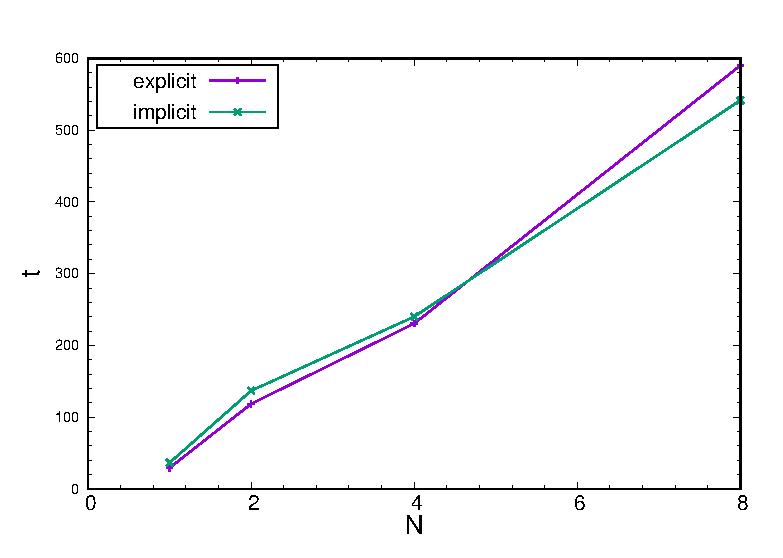
\includegraphics{../plot/time.eps}
    \caption{Time cost}
    \label{fig:time}
\end{figure}

\begin{figure}
    \centering
    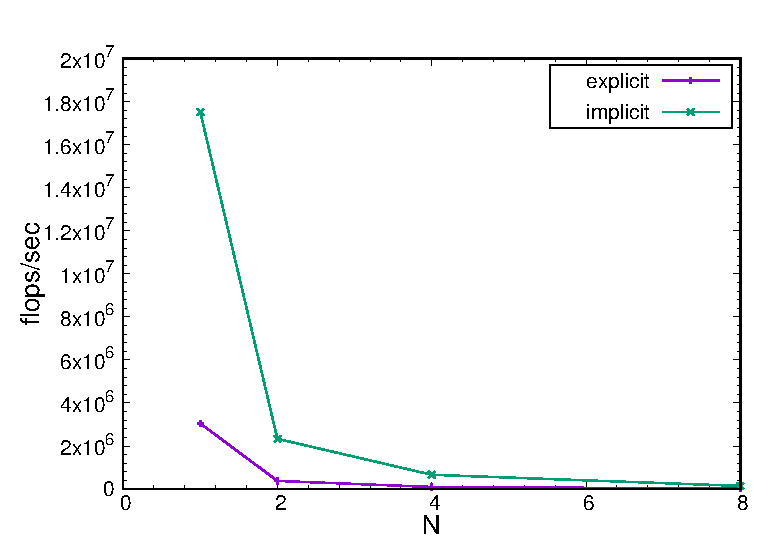
\includegraphics{../plot/flops.eps}
    \caption{Flops/sec}
    \label{fig:flops}
\end{figure}

\end{document}